\documentclass[11pt,letterpaper]{article}
\usepackage[utf8]{inputenc}
\usepackage[spanish,USenglish]{babel}
\usepackage{amsmath}
\usepackage{amsfonts}
\usepackage{amssymb}
\usepackage{amsthm}
\usepackage{graphicx}
\usepackage[left=2cm,right=2cm,top=2cm,bottom=2cm]{geometry}
\usepackage{flushend}
\usepackage{pgf,tikz, pgfplots}
\usetikzlibrary{arrows}
\pgfplotsset{compat=1.15}
\usepackage{pgf,tikz,pgfplots}
%escribir programas
\usepackage{listings}
\usepackage{algpseudocode}
\usepackage{algorithm}
\renewcommand{\algorithmicrequire}{\textbf{Input:}}
\renewcommand{\algorithmicensure}{\textbf{Output:}}

%encabezado
\usepackage{fancyhdr}
\pagestyle{fancy}
\fancyhf{}
\fancyhead[RO]{\thepage} % Números de página en las esquinas de los encabezados
%%%%%%%%%%%%%%%%%%%% BOXES %%%%%%%%%%%%%%%%%%%
\usepackage{bm}
\newcommand{\commentedbox}[2]{%
	\mbox{
		\begin{tabular}[t]{@{}c@{}}
			$\boxed{\displaystyle#1}$\\
			#2
		\end{tabular}%
	}%
}
\usepackage{framed}
\usepackage{wrapfig}\definecolor{shadecolor}{RGB}{224,238,238}
%%%%%%%%%%%%%%%%%%%%%%%%% DEFINITIONS %%%%%%%%%%%%%%%%%%%%%%%%
\theoremstyle{definition}
\newtheorem{defi}{Definición}[section]%Para definiciones
\theoremstyle{definition}
\newtheorem{teo}{Teorema}[section]%Para definiciones
\newtheorem{prop}{Proposición}
\theoremstyle{definition}
\newtheorem{ej}{Ejemplo}[section]
\newtheorem{lem}{Lema}
\newtheorem{prblm}{Problema}
\newtheorem{col}{Corolario}[section]



\title{\textbf{Tarea 6: Embeddings and CNNs}\\ Procesamiento del Lenguaje Natural \\ \Large {Maestría en Computación}\\ \Large {Centro de Investigación en Matemáticas}}
\author{Esteban Reyes Saldaña \\ esteban.reyes@cimat.mx}

\begin{document}

\selectlanguage{spanish}

\maketitle

\section{Paper: Word2Vec}
\begin{enumerate}
	\item \textbf{¿Describa en sus propias palabras la estrategia de selección de palabras dentro de la ventana de contexto en w2v? Expliqué porque se hace así y cual es la intuición.} 
	\\
	La intución es la hipótesis distribucional. Justo por el hecho que la información de una palabra puede ser obtenida viendo las palabras que están a su alrededor (ventanas en este caso). La intución es que en una ventana nos muestra el contexto de una palabara centro. El tamaño de dicha ventana puede variar y a priori se podría decir que entre más grande es la ventana, más información se conoce de la palabra centro. 
	\item \textbf{¿Qué estrategia se usa para construir frases de palabras y construir un solo vector para conceptos basados en más de un token?}	
	\\
	Se identificador un gran número de frases usando una apriximación data-driven. Luego se tratan las frases como tokens individuales durante el entrenamiento. De manera concreta, se identifican las palabras que aparecen frecuentemente juntas y que tienen baja frecuencia en otros contextos. Luego se remplazan por tokens únicos en el conjunto de entrenamiento.
	\item \textbf{¿Según el autor de w2v, cuales podrían ser las diferencias o ventajas/desventajas de CBOW y Skipgram?}
	\\
	Mientras que CBOW predice la palabra actual basada en el contexto, Skip-gram predice palabras cercanas (dentro de la misma oración) dada la palabra actual através de maximizar la clasificación de la palabra actual dada una palabra de la misma oración. Una ventaja/desventaja es que incrementar el rango de Skip-gram mejora la calidad de los embeddings pero también incrementa la complejidad computacional. 
	\item \textbf{¿Cuales son las diferencias entre usar Hierachical Softmax, Negative Sampling y NCE? ¿Cuál recomienda el autor y por qué?}
	\\
	La estructura de Hierachical Softmax está dada por un árbol binario y tiene efectos considerables en el rendimiento del algoritmo. La principal diferencia entre Negative Sampling y NCE es que NCE necesita tanto las muestras como las probabilidades de la distribución del ruido mientras que NS solo usa las muestras. 
	\\
	Dados los resultados del autor, introducir el submuestreo puede resultar en entrenamientos más rápidos y también podría mejorar la exactitud aunque Hierachical Softmax también muestra un buen desempeño.
	\item \textbf{¿Cual diría usted que es la principal conclusión y aportación del paper de w2v? ¿Qué crítica haría usted a estos papers de w2v?}
	\\
	Del primer paper : Los embeddings de las plabaras aprendidas mostraron una estructura lineal que hace posible realizar analogías a través de sumas y restas de vectores Además que realizar submuestreo de palabras frecuentes durante el entrenamiento resulta en mejoras respecto a la velocidad y además, mejora la exatitud de las representaciones de palabras menos frecuentes. 
	\\
	Del segundo paper :	Es posible obtener vectores de alta calidad usando modelos con arquitecturas simples (comparados con modelos de redes neuronales populares). Justo por el bajo costo computacional, es posible entrenar modelos con vectores de palabras de alta dimensionalidad de un conjunto de datos más grande. 	
	\\
	La crítica es sobre la notación y presición matemática al hablar de grupos y usar signos de igual donde no corresponde a una ecuación o una asignación. Por ejemplo, cuando define $ E = 3-50 $ se refiere al rango de $ E $ no a la resta.
\end{enumerate}
%%%%%%%%%%%%%%%%%%%%%%%%%%%%%%%%%%%%%%%%%%%%%%%%%%%%%%%%%%%%%%%%%%
\section{Paper: Glove}
\begin{enumerate}
	\item \textbf{¿Qué desventaja trata de solucionar de W2V?}
	\\
	W2V ha mostrado de manera exitosa capturar finamente la regularidad semántica y sintáctica usando artimética entre vectores pero el origen de dichas regularidades todavía no se ha explicado. Además, Skip-gram utiliza muy poco las estadísticas del corpus (frecuencias) ya que sólo se fija una ventana para el entrenamiento en vez de contar las coocurrencias. 
	\item \textbf{Describa en sus propias palabras y de manera general cual es la principal estrategia para lograrlo.}	
	\\
	Se contruye un modelo para representar palabras que toma en cuenta las co-ocurrencias dentro del corpus. COn la idea de que un punto de inicio aproximado para aprender vectores de palabras debe ser con radios probabilísticos de co-ocurrencia  en vez de la probabilidad en sí.
	\item \textbf{Explique en sus propias palabras las principales conclusiones de los experimentos. Comente si cree que se logró el objetivo.}	
	\\
	GloVe tuvo mejor performance que otros modelos clásicos para vectores de palabras. Se demostró a demás, que se pudo entrenar un corpus con $ 42 $ billones de tokes con un aumento sustancial del rendimiento correspondiente. Finalmente, para GloVe, el parámetro relevante es es el número de iteraciones en el entrenamiento mientras que para $ wor2vec $ y de manera análoga para $ word2vec $ la elección obvia sería el número de épocas de entrenamiento.
	\item \textbf{¿Encuentra alguna relación entre Glove y las clasicas TCOR y DOR? ¿Cuales?}
	\\
	Sí. TCOR, DOR y GloVe se basan en la matriz de co-ocurrencias de las palabras en un corpus dado. De hecho GloVe utiliza la matriz de co-ocurrencias entre palabras para encontrar las representaciones vectoriales.
	\item \textbf{¿Cual diría usted que es la principal conclusión y aportación del paper de Glove? ¿Qué crítica haría usted a estos papers de Glove?}	
	\\
	GloVe produce un espacio de vectores con un desempeño mejor que otros algoritmos en el estado del arte, pero con tamaños de vectores más pequeños y con corpus más pequeños. Concluyen también que los vectores obtenidos por GloVe son útiles para otras tareas de NLP. 
	\\
	Al igual que $ word2vec $, la notación matemática. Cuando comienza a definir las funciones $ F(\cdot) $ no se refiere a una asignación o un igual, si no a una función que represente dichos parámetros.
\end{enumerate}
\section{Otros papers}
\begin{enumerate}
	\item \textbf{¿Qué desventaja trata de solucionar FastText y cómo lo logra?}
	\\
	Los algoritmos más populares para obtener representaciones vectoriales de palabras ignoran la morfología de las palabras asignando vectores distintos a cada palabra. Lo cual podría ser una desventaja para corpus de un idioma con vocabularios largos. Para solucionar esto, se propone una implementación del modelo Skip-gram donde cada palabra se representa (usando información a nivel de caracter) como una bolsa de n-gramas.
	\item \textbf{¿Cuál sería la principal desventaja de FastText vs Word2Vec?}	
	\\
	Para los experimentos muchas de las palabras de los datasets no aparecieron en los datos de entrenamiento y por lo tanto, no se pudo obtener una representación vectorial de dicha paralara usando $ cbow $ o $ skipgram $.
	\\
	Además, se tuvieron problemas de rapidez de convergencia comparado con $ skipgram $ dada su implementación de bajo nivel en $ C $.
	\item \textbf{¿Qué desventaja trata de solucionar el paper de Directional W2V y cómo lo logra? Describa brevemente las conclusiones de la sección experimental.}	
	\\
	Los modelos base, como $ skip-gram $, no distinguen explícitamente las ventanas a la izquierda o a la derecha de una palabra dada. Además, las implementaciones se restringuen para proporcionar dicha información, dado que la capa oculta de una red neuronal requiere ser más grande o pesos adicionales. Para solucionar esto, se propone una adaptación del modelo $ SD $ que considera no solo los patrones de co-ocurrencia si no también la posición relativa de una palabra mediante una función $ sofmax $ que mide cuánto contexto de una palabra está asociada con los elementos a la izquierda y a la derecha.
	\\
	Sobre los experimentos, se realizaron evaluaciones intrínsecas e intrínsecas, tales como velocidad de entrenamiento, similaridad de palabras y speach-tagging. Se encotró que, comparado con el modelo original, $ SG $, este modelo obtiene una mejor velodiad de caída cuando se aumenta el tamaño de la ventana de contexto. Además, para la tarea de pos-tagging este modelo captura de manera efectiva la información sintáctica.
	\item \textbf{¿Qué se dice acerca del análisis de complejidad del Directional w2v?}
	\\
	En comparación con el modelo original $ SD $, este modelo sólo requiere una operación extra. Luego, aumentar el tamaño de la ventana significa tener velocidades similares al modelo $ SG $. Mientras que modelos como el $ SSG $ decrece en manera considerable al aumentar el tamaño de la ventana.
	\item \textbf{En el paper de gnome-mining, ¿Qué técnicas de NLP son usadas y con que objetivo intuitivo cada una?}
	\\
	Se usa la representación vectorial de palabras y redes neuronales recurrentes. De manera intuitiva, para capturar información de dependencia en términos cortos y largos. Luego se usa la similaridad respecto al coseno para comparar los vectores en el dominio.
	\item \textbf{¿En que problemas de clasicación evaluó Kim su CNN?}
	\\
	Revisiones de películas, Stanford Sentiment Treebanck, clasificacipon de oraciones como subjetivas u objetivas, clasificación de preguntas, clasificación de opiniones de consumidor.	
	\item \textbf{En los resultados dónde estuvo involucrado algún método de clasicación con SVM, ¿Cómo fue el resultado respecto a CNNs? ¿Qué features usaba el método basado en SVM?}
	\\
	El resultado fue superior en términos de accuracy para todas las configuraciones de las $ CNN $. Los features usados en $ SVM $ fueron : unigramas, bigramas, trigramas, palabra wh, head word, POS, parser, hiperónimos, y $ 60 $ regla escritas a mano.
	\item \textbf{En sus propias palabras, ¿Qué diferencia tienen las estrategias multi-channel y single-channel?, ¿Cuál recomienda Kim?}
	\\
	Multi-channel utiliza dos pares de embeddings en los cuales sólo uno de ellos va cambiando con el descenso gradiente mientras que el otro se mantiene para no sobre entrenar al modelo con el dataset. 
	\\
	Recomienda usar single-channel fijo pero con dimensiones extra que se puedan modificar durante el entrenamiento.
	\item \textbf{¿Cual diría usted que es la principal conclusión y aportación del paper de Kim? ¿Qué crítica le haría usted a Kim? }		
	\\
	Una red $ CNN $ simple con embeddings estáticos alcanza resultados excelentes en distintas tareas. Sus resultados sugieren que los vectores pre-entrenados son características universales que se pueden utilizar para distintos datasets. Finalmente, una fina modificación a estos vectores muestra mejoras en los resultados.
\end{enumerate}

\section{CNNs}
Estudie supercialmente el siguiente notebook:
\\ https://github.com/fagonzalezo/dl-tau-2017-2/blob/master/Handout-CNN-sentence-classification.ipynb 
\\
En esta tarea se le pro-
porcionará el CNN-rand pero en Pytorch. Investigue lo necesario para completar el CNN-static y el CNN-non-static por usted mismo. Contruya la gŕafica de comparación de los tres.
\begin{center}
	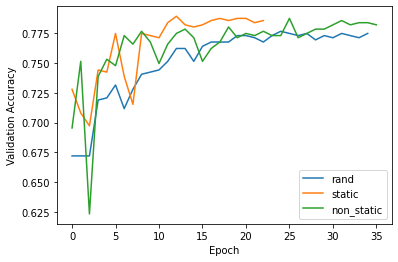
\includegraphics[width=0.7\linewidth]{comparation_cnn}
\end{center}
\end{document}